\section{Affine Copies and the Self Similarity Property}

One of the more popularly known results from math is the the Mandelbrot set fractal.  In some senses fractals can be very general objects that are considered to have fractional dimensions.  This definition can be very general but by that same token, may not always capture some of the inherent geometry of some fractal type objects. Some objects with fractional dimensions have a self-similar property, and some self-similar objects have fractional dimension.  For the scope of this paper, we will not be discussing dimension. However we will investigate the notion of self-similarity. 


Even one dimensional objects can have this self-similar property. Take for example the middle Third Cantor set.  The middle third Cantor set is defined by recursively removing the open middle third interval of the previous remaining closed intervals.  Explicitly this can be constructed using countable intersection.  

\begin{example}[The Middle Third Cantor Set]\label{middleThirdCantor}
    $$\mathcal{C} = [0,1] \setminus \bigcup_{n=0}^\infty\bigcup_{k=0}^{3^n-1}\left(\frac{3k+1}{3^{n+1}},\frac{3k+2}{3^{n+1}}\right)$$
\end{example}

This set in particular exhibits this self-similar property because each level is a scaled copy of the entire object.  The following figure shows the first seven intervals removed.  

\begin{figure}[h]
    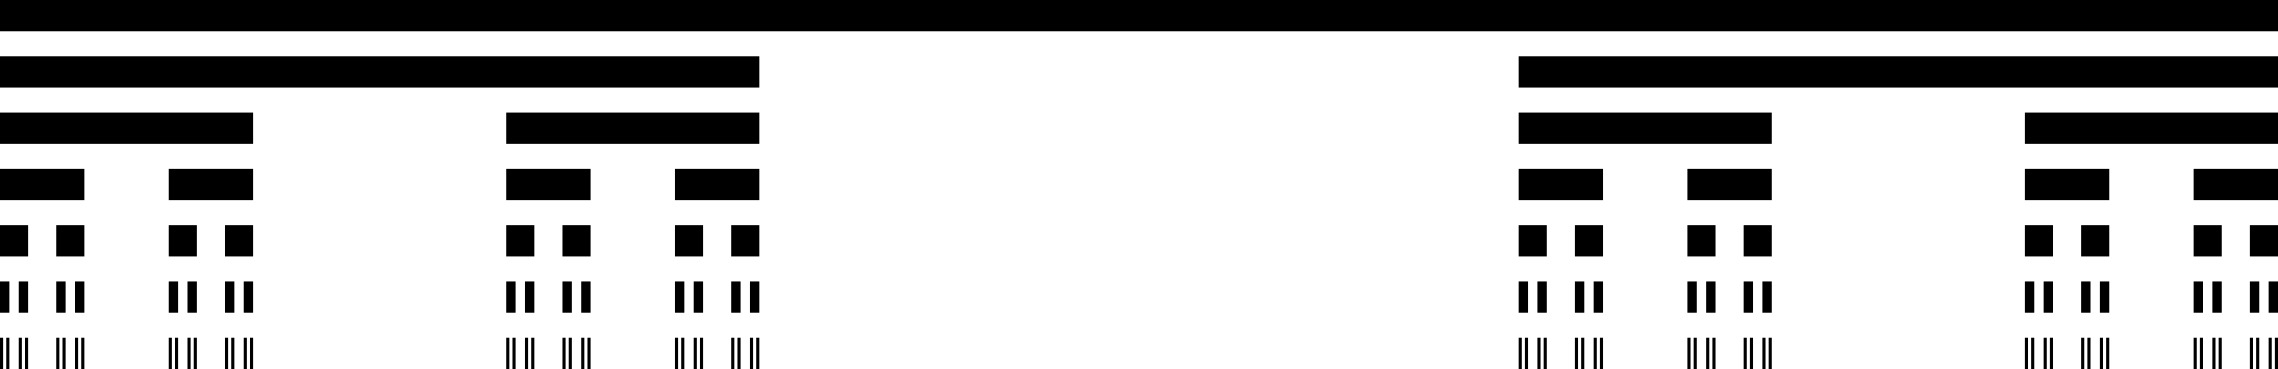
\includegraphics[width=0.8\textwidth]{Content/Images/Cantor_set_in_seven_iterations.jpg}
    \centering
    \caption{The first seven iterations of the middle third Cantor Set.}
\end{figure}
In a general sense, we can take a set, then dilate and translate a copy of it. 

\begin{definition}[Dilation]\cite{GEdgar}
    Let $r>0$ and $a \in \R$.  The \underline{dilation} on $\R$ with ratio $r$ and center $a$ is the function $f: \R \to \R$ given by $$f(x)= rx + (1-r) a.$$
\end{definition}

Now we consider the following two dilation funcitons each with the contraction ratio 1/3: 
$$f_1 (x) = \frac{1}{3}x \quad \text{ and } \quad f_2 (x) = \frac{x+2}{3}.$$


We will use these two to demonstrate that the Cantor set is self-similar.  This is an example of the definition of self similar, the collection of invariant points under iterated function systems.  In this case the two functions are the iterated funciton system and the set of invariant points is the Cantor set.  Admittedly this is an abstract definition so here is a proposition to work through the specific mechanics.  

\begin{proposition}The Cantor set is self-similar.   That is to say the Cantor set satisfies the self-referential equations 
    $$\mathcal{C} = f_1 [\mathcal{C}] \cup f_2 [\mathcal{C}].$$
\end{proposition}
\begin{proof}
    Recall the definition of the Cantor set, as the iterated removal of the middle third.      
    $$\mathcal{C} = [0,1] \setminus \bigcup_{n=0}^\infty\bigcup_{k=0}^{3^n-1}\left(\frac{3k+1}{3^{n+1}},\frac{3k+2}{3^{n+1}}\right)$$

    Here we notice that for the first removal, $n = 0$, we are left with the left and right portion of the Cantor set.  Specifically the left side is a translated copy of the right side:

    \begin{align*}
        \left[\frac{2}{3},1\right] \setminus \bigcup_{n=1}^\infty\bigcup_{k=0}^{3^n-1}\left(\frac{3k+1}{3^{n+1}},\frac{3k+2}{3^{n+1}}\right) &= \underbrace{ \left\{\left[0,\frac{1}{3}\right] \setminus \bigcup_{n=1}^\infty\bigcup_{k=0}^{3^n-1}\left(\frac{3k+1}{3^{n+1}},\frac{3k+2}{3^{n+1}}\right)\right\} }_{\text{the left side of the cantor set}}  + \frac{2}{3}\\
        &= \underbrace{ \frac{1}{3}\left\{[0,1] \setminus \bigcup_{n=0}^\infty\bigcup_{k=0}^{3^n-1}\left(\frac{3k+1}{3^{n+1}},\frac{3k+2}{3^{n+1}}\right)\right\} }_{\text{the left side of the cantor set}}  + \frac{2}{3} \\
        &= \frac{1}{3}\left\{ \underbrace{ [0,1] \setminus \bigcup_{n=0}^\infty\bigcup_{k=0}^{3^n-1}\left(\frac{3k+1}{3^{n+1}},\frac{3k+2}{3^{n+1}}\right) }_{\text{the original Cantor set}} \right\}   + \frac{2}{3} \\
        &=f_2 [\mcC] 
    \end{align*}

    We note that this happens at every level of the cantor set.  In otherwords by induction:
    $$\mcC_{n+1} = f_1[\mcC_n] \cup f_2 [\mcC_n].$$

    Notice that by using the above two equations, the Cantor set satisfies the self-referential equations:
    $$\mathcal{C} = f_1 \mathcal{C} \cup f_2 \mathcal{C}.$$


\end{proof}
\begin{definition}[Iterated Function System]
    An iterated function system is a finite set of contraction mappings on a complete metric space.  Symbolically, we write this as, for some $N \in \N$,
    $$\{f_i:X \to X \vert i = 1,2,\dots, N\}, $$
\end{definition}

\begin{definition}[Self-Similar Set]
    A set $A$ is self-similar if it is the invariant set of an iterated function system. 
\end{definition}


The invariant set under this iterated function system is a self similar set.